\begin{table*}[t]
\centering
\scriptsize
\setlength{\tabcolsep}{3.4pt}
\renewcommand{\arraystretch}{1.15}
\caption{Comparison with representative executable GUI-agent benchmarks. OS-OMNI covers desktop, mobile, web, and cross-platform workflows, enabling unified evaluation of generalist GUI agents across heterogeneous operating systems and applications.}
\label{tab:benchmark_comparison}
\resizebox{\textwidth}{!}{
\begin{tabular}{lccccccccccc}
\toprule
\multirow{2}{*}{\textbf{Benchmark}} &
\multirow{2}{*}{\makecell{\textbf{\# Tasks} \\}} &
\multicolumn{6}{c}{\textbf{Platform}} &
\multirow{2}{*}{\makecell{\textbf{Cross-} \\ \textbf{Platform}}} &
\multirow{2}{*}{\makecell{\textbf{Cross-} \\ \textbf{App}}} &
\multirow{2}{*}{\makecell{\textbf{Curated} \\ \textbf{Apps}}} &
\multirow{2}{*}{\makecell{\textbf{\# Apps} \\ \textbf{/ Sites}}} \\
\cmidrule(lr){3-8}
& &
\textbf{Win.} &
\textbf{Linux} &
\textbf{macOS} &
\textbf{iOS} &
\textbf{Android} &
\textbf{Web} &
& & & \\
\midrule

WorkArena~\citep{drouin2024workarena} &
33 &
\xmark & \xmark & \xmark & \xmark & \xmark & \cmark &
\xmark &
\xmark &
\xmark &
1 \\

WebArena~\citep{zhou2023webarena} &
812 &
\xmark & \xmark & \xmark & \xmark & \xmark & \cmark &
\xmark &
\xmark &
\xmark &
6 \\

VisualWebArena~\citep{koh2024visualwebarena} &
910 &
\xmark & \xmark & \xmark & \xmark & \xmark & \cmark &
\xmark &
\xmark &
\xmark &
3 \\

AndroidWorld~\citep{rawles2024androidworld} &
116 &
\xmark & \xmark & \xmark & \xmark & \cmark & \xmark &
\xmark &
\cmark &
\xmark &
20 \\

WindowsAgentArena~\citep{bonatti2024windows} &
154 &
\cmark & \xmark & \xmark & \xmark & \xmark & \cmark &
\xmark &
\cmark &
\xmark &
11 \\

AssistGUI~\citep{gao2023assistgui} &
100 &
\cmark & \xmark & \xmark & \xmark & \xmark & \xmark &
\xmark &
\xmark &
\xmark &
9 \\

WorldGUI~\citep{zhao2025worldgui} &
611 &
\cmark & \xmark & \xmark & \xmark & \xmark & \cmark &
\xmark &
\xmark &
\xmark &
10 \\

macOSWorld~\citep{yang2025macosworld} &
202 &
\xmark & \xmark & \cmark & \xmark & \xmark & \xmark &
\xmark &
\cmark &
\xmark &
30 \\

OSWorld~\citep{xie2024osworld} &
369 &
\cmark & \cmark & \cmark & \xmark & \xmark & \cmark &
\xmark &
\cmark &
\xmark &
9 \\

ScienceBoard~\citep{sun2025scienceboard} &
169 &
\xmark & \cmark & \xmark & \xmark & \xmark & \xmark &
\xmark &
\cmark &
\xmark &
6 \\

MMBench-GUI~\citep{wang2025mmbench} &
967 &
\cmark & \cmark & \cmark & \xmark & \cmark & \cmark &
\xmark &
\cmark &
\xmark &
-- \\

OS-MAP~\citep{chen2025map} &
416 &
\xmark & \cmark & \xmark & \xmark & \xmark & \cmark &
\xmark &
\cmark &
\xmark &
15 \\

\midrule
\textbf{OS-OMNI} &
\textbf{1200} &
\cmark & \cmark & \cmark & \cmark & \cmark & \cmark &
\cmark &
\cmark &
\cmark &
\textbf{35} \\
\bottomrule
\end{tabular}
}
% \vspace{0.3em}
\begin{flushleft}
\scriptsize
% \textbf{Note.} \cmark: supported; \xmark: not supported; \textbf{P}: partial support. ``Cross-Platform'' denotes workflows that span multiple operating systems or runtime environments, rather than merely evaluating separate tasks on different platforms. ``Curated Apps'' denotes benchmark-controlled applications or services with reproducible account/service state and final-state evaluation. Partial support indicates reliance on external real-account login or preloaded local account/profile state rather than benchmark-controlled account-service backends.
\end{flushleft}
\end{table*}


\begin{figure}[t]
    \centering
    \makebox[\textwidth][c]{%
        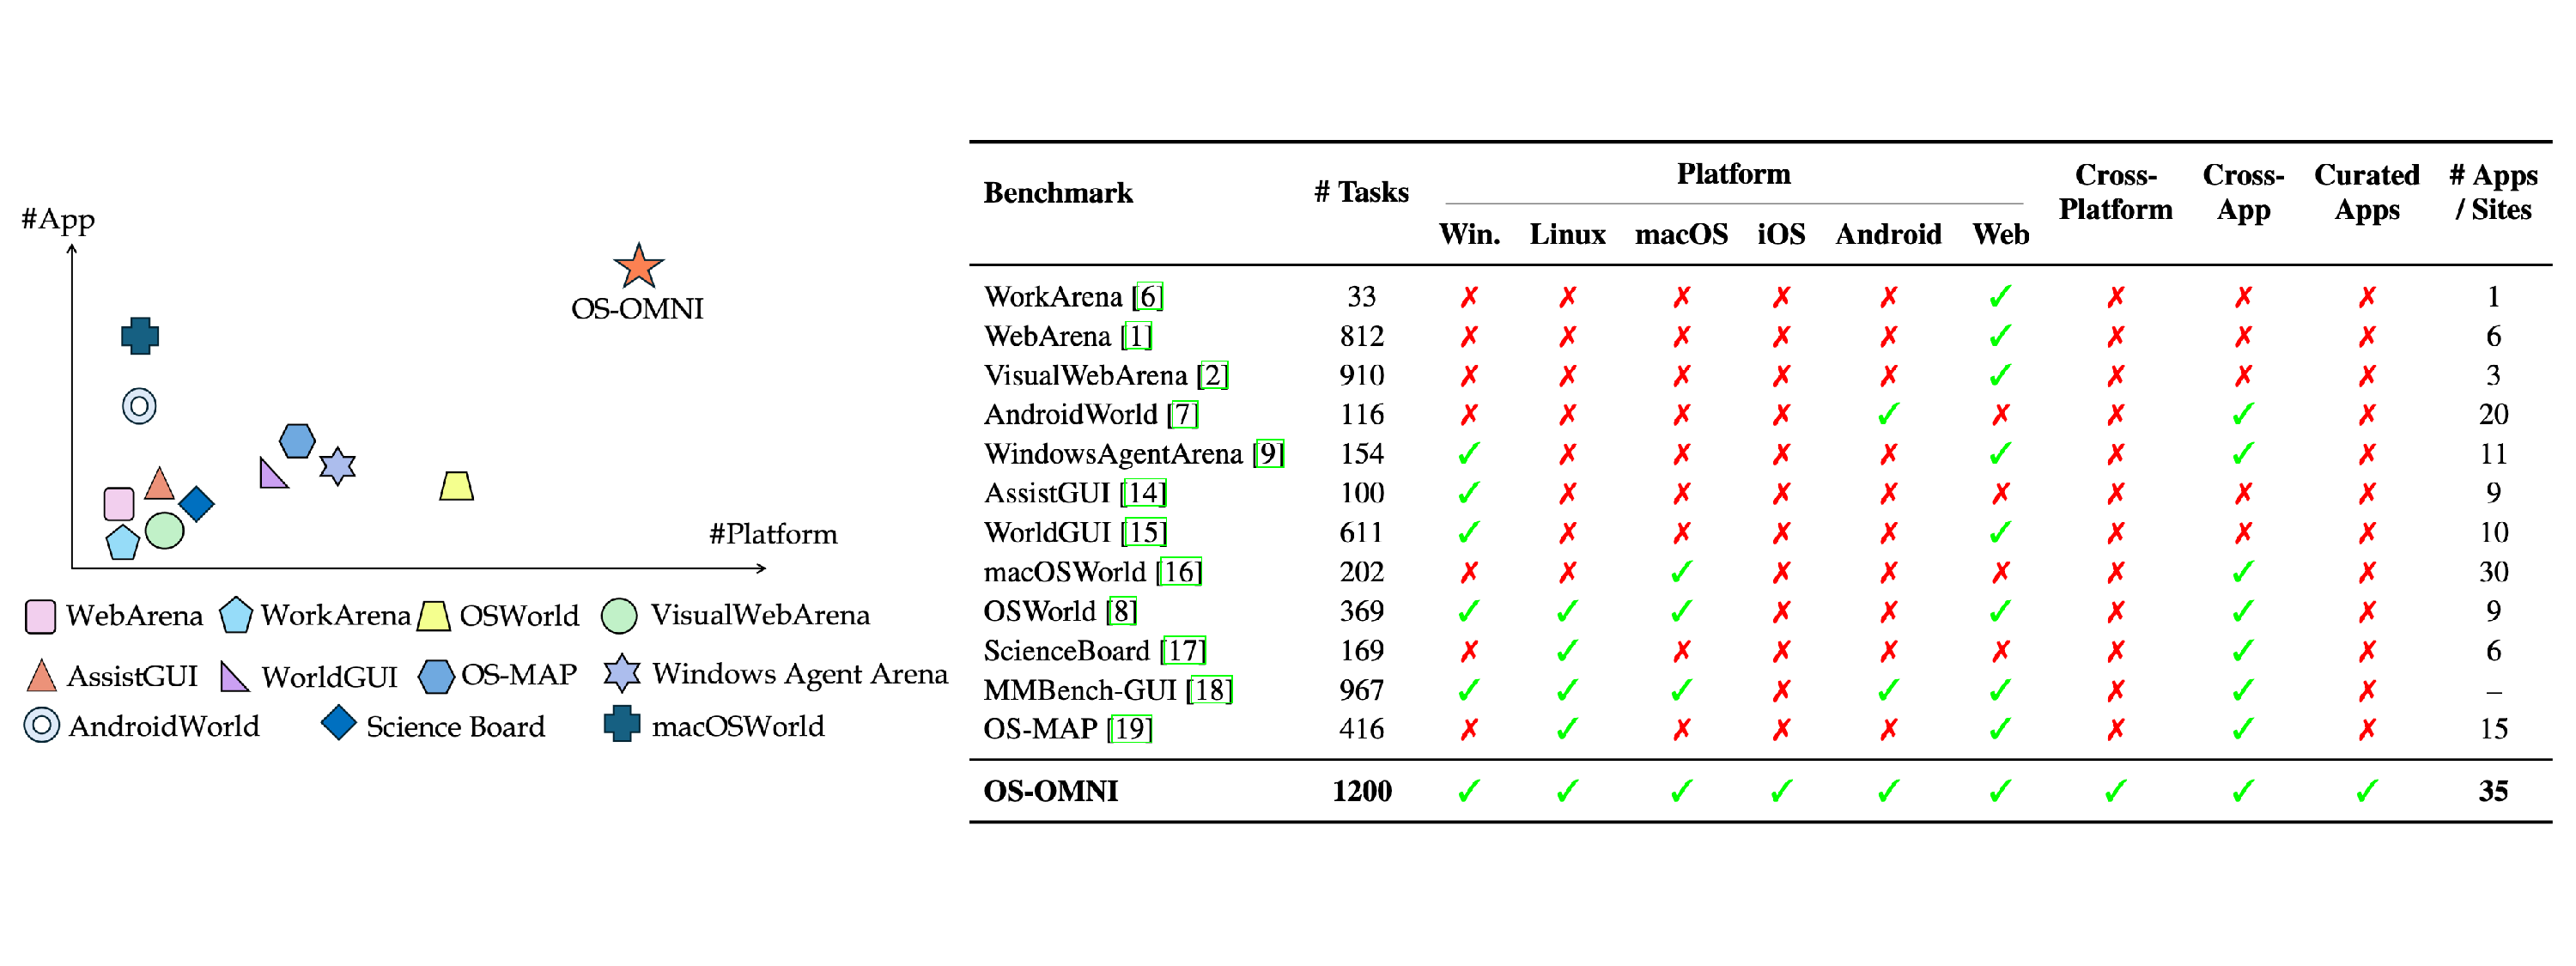
\includegraphics[width=1.2\textwidth]{figures/table1.pdf}
    }
    \caption{
Comparison with representative executable GUI-agent benchmarks. 
\#Platform indicates the number of supported platforms among Windows, Linux, macOS, iOS, Android, and Web, and \#App indicates the number of covered applications or websites. 
% For task properties, Cross-Platform denotes workflows spanning multiple operating systems or runtime environments, Cross-App denotes coordination across multiple applications, and Curated Apps denotes benchmark-controlled applications or services with reproducible account or service state and final-state evaluation. 
Compared with existing benchmarks, OS-OMNI provides broader platform coverage, richer application diversity, cross-platform workflows, and curated account-based service evaluation.
}
    \label{fig:comparison_benchmarks}
\end{figure}